\chapter{Realisieren} \label{ch:implement}

Gestützt auf den vorherigen Phasen der gewählten Projektmanagementmethode wird in diesem Kapitel die eigentliche Implementation des Systems dokumentiert.
Diese wird bezogen auf den Arbeitsprozess möglichst linear und strukturiert wiedergegeben.

\section{Versionierung und Backups} \label{sec:backups}

\subsection{Code}

Die Ruby on Rails Applikation wird gemäss Renuo-Guidelines in einem Git-Repository auf GitHub versioniert. Es werden keine Pull Requests erstellt,
da diese für eine Einzelarbeit in dieser Grösse keinen Nutzen von sich tragen. Stattdessen wird versucht, eine möglichst saubere History zu schaffen mit kurzen, aussagekräftigen Git Commit-Messages.
So ist der Verlauf der Arbeit gut nachvollziehbar und es kann jederzeit auf eine vergangene Version zurückgegriffen werden. Nach jedem Commit
wird dieser direkt auf den remote \emph{develop} Branch gepusht.

\begin{figure}[H]
    \centering
    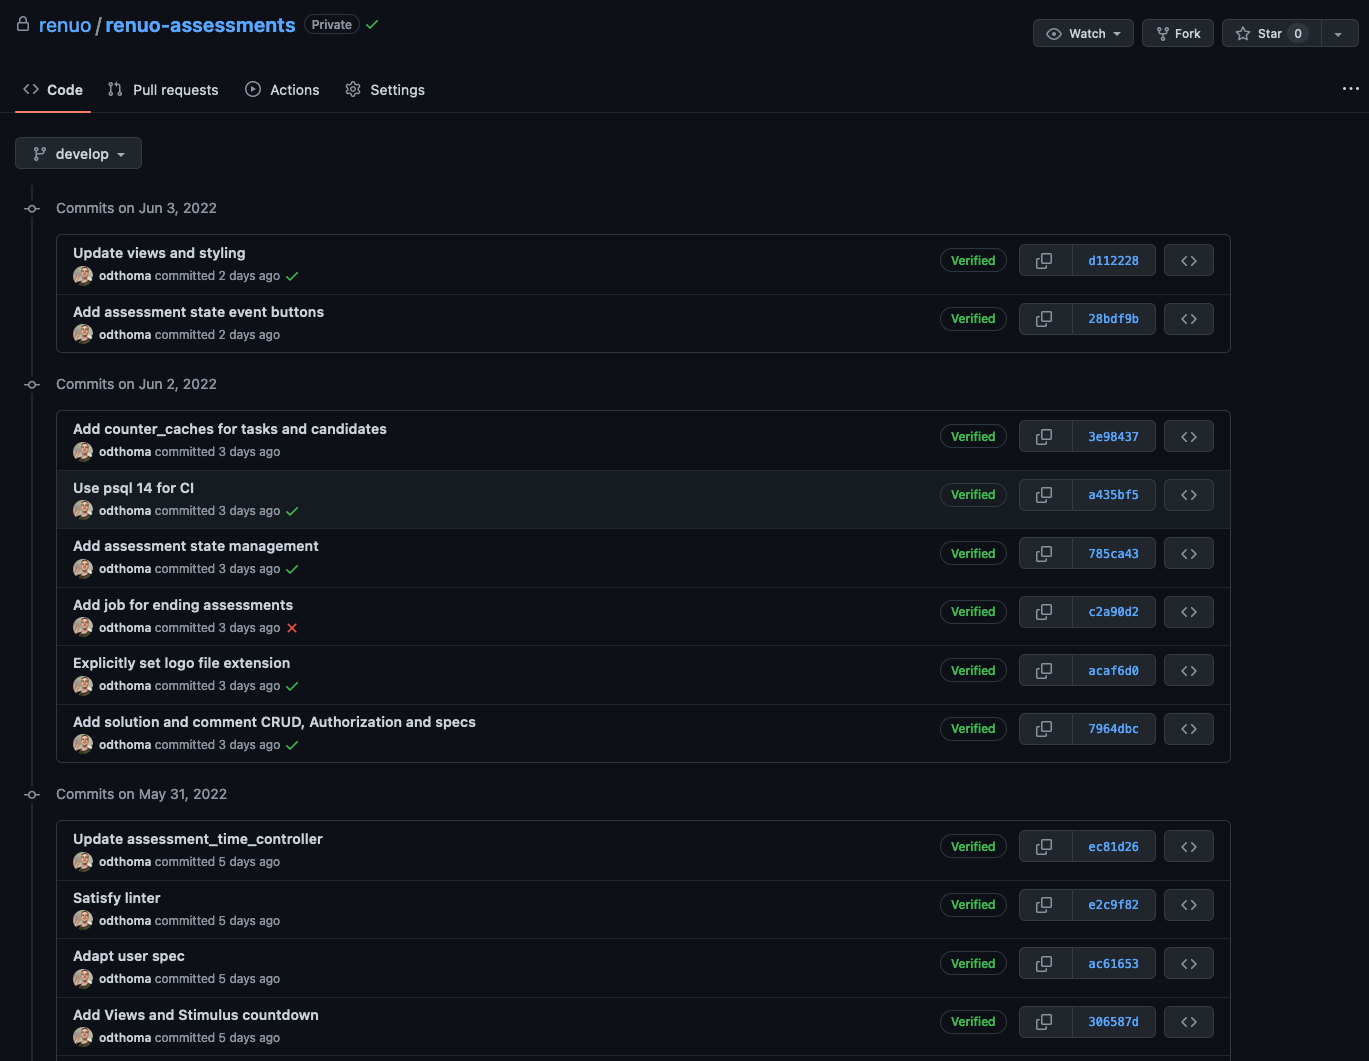
\includegraphics[width=14cm]{images/renuo-assessments-github.png}
    \caption{\label{fig:renuo-assessments-github}Ausschnitt der GitHub Commit-History vom Ruby on Rails Projekt}
\end{figure}

\newpage

\subsection{IPA-Bericht}

Das LaTeX Projekt wird ebenfalls in einem Git-Repository versioniert und es werden zu sinnvollen Zeitpunkten Commit gemacht. Diese werden dann regelmässig auf ein Remote (GitHub) gepusht und es wird jeden Abend ein neuer Git-Tag erstellt.
In dem Repository befinden sich alle Diagramme und sonstigen Dateien, die für die Umsetzung des IPA-Berichtes notwendig sind. 
So ist eine rasche Wiederherstellung der aktuellen Daten im Falle eines Datenverlustes jederzeit und von überall aus möglich.

\begin{figure}[H]
    \centering
    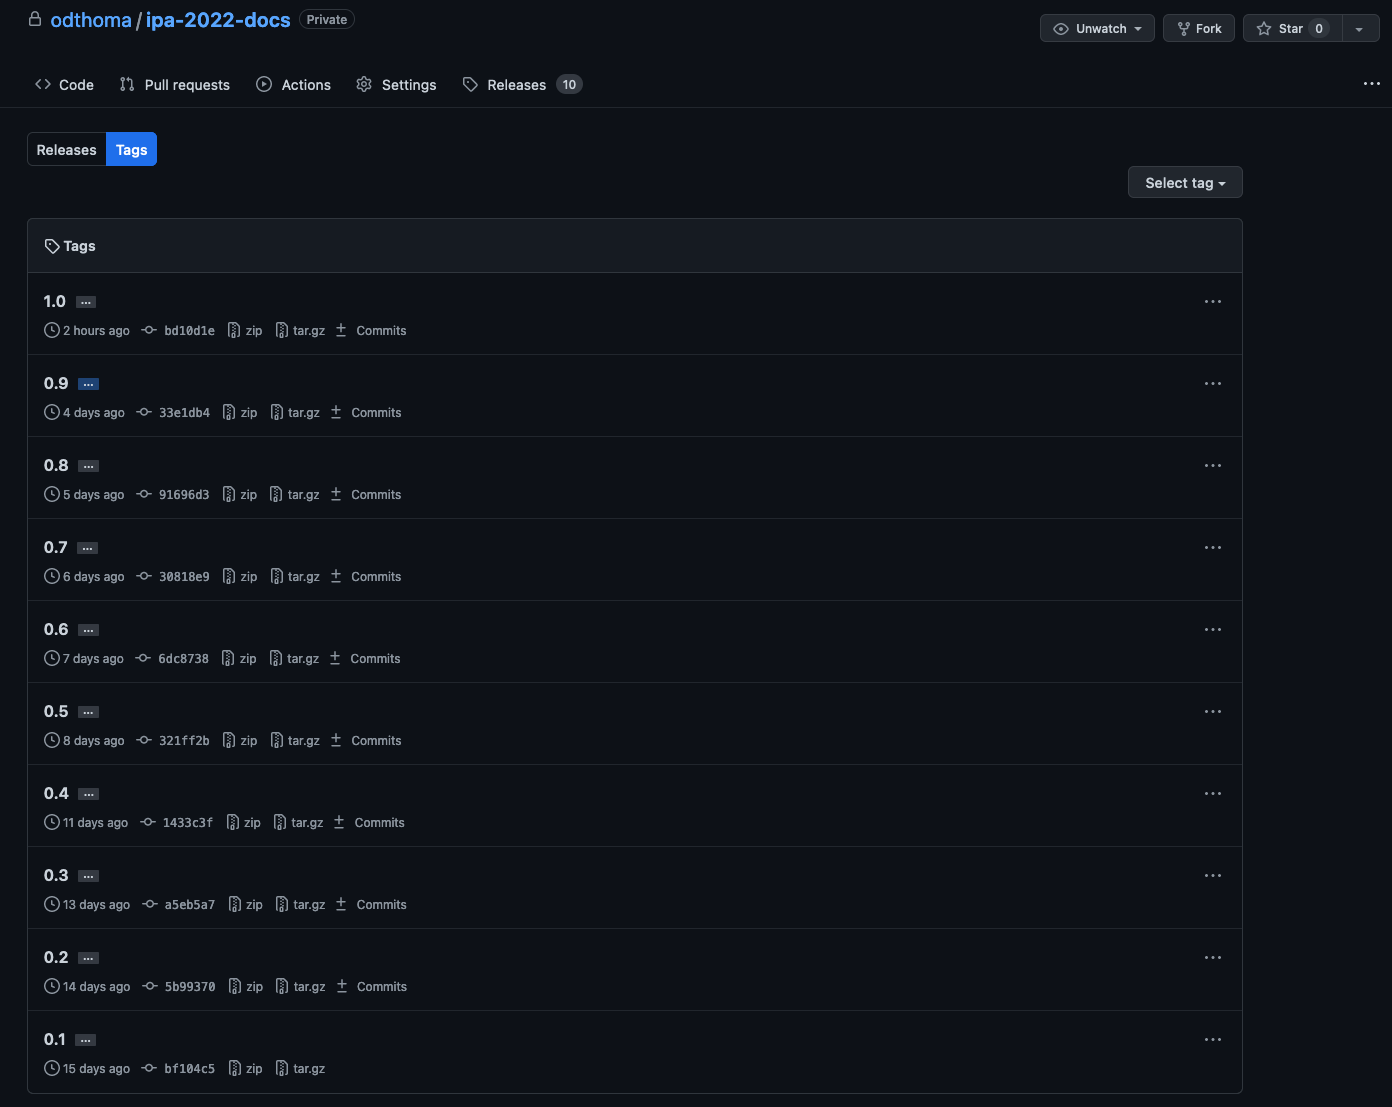
\includegraphics[width=14cm]{images/latex-github-tags.png}
    \caption{\label{fig:latex-github-tags}Tägliche Versionierung des IPA-Berichts über Git-Tags}
\end{figure}


\newpage


\section{Authentifizierung}

Als Authentifizierungssystem wird das \enquote{Devise} gem eingesetzt. Dies ist eine sehr bekannte, vollumfängliche Lösung für Ruby on Rails,
welche einem die ganze Arbeit abnimmt, ein solches System selbst zu implementieren. Durch die mitgelieferten Generator-Commands
kann schnell eine stabile Grundstruktur geschaffen werden - sogar inklusive allen HTML-Templates, welche nur noch leicht angepasst werden mussten. 
Die notwendigen Model-Klassen und Datenbankmigrationen werden so ebenfalls vollautomatisch generiert.

\begin{codebox}
\begin{minted}{shell}
rails generate devise:install
rails generate devise User
rails generate devise:views

rails db:migrate # führt die generierten ActiveRecord Migrationen aus
\end{minted}
\end{codebox}

Devise basiert auf sogenannten \enquote{Strategies}, welche im User-Model definiert werden. Diese beschreiben,
welche Funktionalitäten von Devise aktiviert werden sollen und welche nicht.

\begin{codebox}
\begin{minted}{ruby}
class User < ApplicationRecord
  devise :database_authenticatable, :recoverable, :trackable
          :confirmable, :rememberable, :validatable, :registerable
end
\end{minted}
\end{codebox}

Hier wird auch die \mintinline{ruby}{:registerable} Strategy aufgelistet, die einen Registrierungsprozess implementiert.
Und das, obwohl keine selbstständigen Registrierungen möglich sein sollten, da Bewerber nur per Einladungs-Link an einem Assessment teilnehmen können. 
Die Strategy wird hier allerdings bewusst eingesetzt, da sie auch ein Formular für das Ändern von E-Mail-Adresse und Passwort bietet. 
Das eigentliche Registrierungsformular \emph{/user/registrations/new} wird dann einfach explizit über die Devise route-definition deaktiviert, während
die edit-routes manuell eingetragen werden.

\begin{codebox}
\begin{minted}{ruby}
Rails.application.routes.draw do
  devise_for :users, skip: %i[registrations]

  devise_scope :user do
    get 'users/edit', to: 'devise/registrations#edit'
    put 'users', to: 'devise/registrations#update'
  end

  ...
end
\end{minted}
\end{codebox}

Ausserdem werden Strategies eingesetzt um:
\begin{enumerate}
  \item Passwörter via E-Mail zurückzusetzen
  \item Jeden login/logout zu protokollieren inkl. Zeit, Datum, IP-Adresse
  \item Formulareingaben zu validieren
  \item Nach einer Änderung der E-Mail-Adresse diese via Link zu bestätigen
\end{enumerate}


\section{Umsetzung der Datenstruktur}

Die grundlegende Datenstruktur wurde anhand der vordefinierten Rails-Generator Commands \ref{subsec:model-generation} aufgebaut.
Damit war der grösste Teil der Arbeit bereits erledigt und es mussten lediglich die Assoziationen in den jeweiligen Model-Klassen ergänzt werden.
Diese werden dort durch die ActiveRecord Funktionen \mintinline{ruby}{has_many}, \mintinline{ruby}{has_one}, und \mintinline{ruby}{belongs_to} abgebildet.

Zwischen der \emph{user} und \emph{assessment} Tabelle herrscht eine many-to-many Assoziation, da ein Bewerber mehrere Assessments haben kann, 
woran wiederum mehrere Bewerber teilnehmen können. Dafür wird die Join-Tabelle \emph{assessment\_participations} eingesetzt. 
Um nun sicherzustellen, dass ein Bewerber nur einmal in einer Assessment-Instanz vorkommen kann, wurde über eine ActiveRecord Datenbankmigration ein 
unique composite Index über beide Fremdschlüssel erstellt.

\begin{codebox}
\begin{minted}{ruby}
def change
  add_index :assessment_participations, %i[user_id assessment_id], unique: true
end

\end{minted}
\end{codebox}

Ausserdem sollte ein Bewerber nur eine einzige Lösung pro Aufgabe abgeben können. Dafür wurde auf der \emph{solutions}
Tabelle ebenfalls ein unique composite Index erstellt. Beide Indizes werden auch auf Application-Level in den entsprechenden Model-Klassen
durch Validierungen abgesichert, wodurch lesbarere Error-Messages für die Formulare im Frontend generiert werden können.

\begin{codebox}
\begin{minted}{ruby}
def change
  add_index :solutions, %i[user_id task_id], unique: true
end
\end{minted}
\end{codebox}

\begin{codebox}
\begin{minted}{ruby}
class Solution < ApplicationRecord
  belongs_to :task
  belongs_to :user
  has_many :comments, dependent: :destroy

  validates :user_id, uniqueness: { scope: :task_id }

  ...
end
\end{minted}
\end{codebox}

\begin{codebox}
\begin{minted}{ruby}
class AssessmentParticipation < ApplicationRecord
  belongs_to :assessment
  belongs_to :user

  validates :user_id, uniqueness: { scope: :assessment_id }

  ...
end
\end{minted}
\end{codebox}

\newpage

\section{CRUDs}

Bei Ruby on Rails handelt es sich um ein \gls{mvc} Framework. Daher wurde für alle generierten Model-Klassen
auch eine Controller-Klasse und die entsprechenden HTML-Views erstellt. Diese folgen grösstenteils dem Rails-Standard \cite{default_controller_actions} und beinhalten einfache \gls{crud} Operationen.
Basierend auf der Aufgabenstellung wurden nicht für jede Ressource alle vier Operationen implementiert.

Die Funktionen in einem Rails ActionController werden \enquote{Actions} genannt. Der folgende Codeausschnitt zeigt zwei dieser Actions,
die die Erstellung eines Assessments implementieren. Ein wichtiges Konzept hierbei sind die \emph{ActionController::StrongParameters}.
Durch diese werden die Anzahl der Felder, die bei der Erstellung eines Assessments mitgegeben werden können, limitiert. Auch dieses
Sicherheitskonzept wurde in allen Controllern implementiert.

\begin{codebox}
\begin{minted}{ruby}
class AssessmentsController < ApplicationController
  def new # GET /assessments/new
    @assessment = Assessment.new
  end

  def create # POST /assessments
    @assessment = Assessment.new(assessment_params)
    if @assessment.save
      redirect_to assessment_path(@assessment)
    else
      render :new, status: :unprocessable_entity
    end
  end

  ...

  private

  def assessment_params
    params.require(:assessment).permit(:title, :starts_at, ...)
  end
end
\end{minted}
\end{codebox}

Nachdem eine Action durchlaufen ist und kein HTML-Template explizit gerendert wurde, sucht sich das Framework automatisch
ein Template mit dem entsprechenden Namen und rendert dieses. So wird beispielsweise in der 
oberhalb gezeigten \emph{new} Action eine Instanzvariable gesetzt und dann automatisch das \emph{views/assessments/new.html.slim} HTML-Template gerendert.
Diese Instanzvariable kann dann in den Templates verwendet werden.

So wurden für alle notwendigen Models, sprich \emph{Assessment}, \emph{Task}, \emph{Solution} und \emph{Comment} mit der Hilfe des \enquote{simple\_form} Gems
die notwendigen Formulare erstellt.

\begin{codebox}
\begin{minted}{ruby}
= simple_form_for @assessment do |f|
    = f.input :title
    = f.input :starts_at
    = f.button :submit
\end{minted}
\end{codebox}


\section{Routing}

\section{Autorisierung}

\subsection{Benutzerrollen}

Die Rolle eines Benutzers wird im User-Model in Form eines \emph{ActiveRecord::Enum} abgebildet. Hier wird bewusst ein Sting-Wert in der Datenbank
bevorzugt, da sich ein Integer-Wert beim Hinzufügen von neuen Rollen verändern könnte. Ausserdem ist so in der Datenbank die Benutzerrolle immer
direkt ersichtlich. Auf den Enum wird auch der Default-Wert \enquote{candidate} gesetzt, sodass neue Benutzer, die eingeladen werden, automatisch dieser Rolle zugeteilt werden. 

\begin{codebox}
\begin{minted}{ruby}
class User < ApplicationRecord
  enum :role, { admin: 'admin', candidate: 'candidate' }, default: :candidate
end
\end{minted}
\end{codebox}

Die Benutzerrolle kann dann auf jeder User-Instanz folgendermassen abgerufen werden:

\begin{figure}[H]
  \centering
  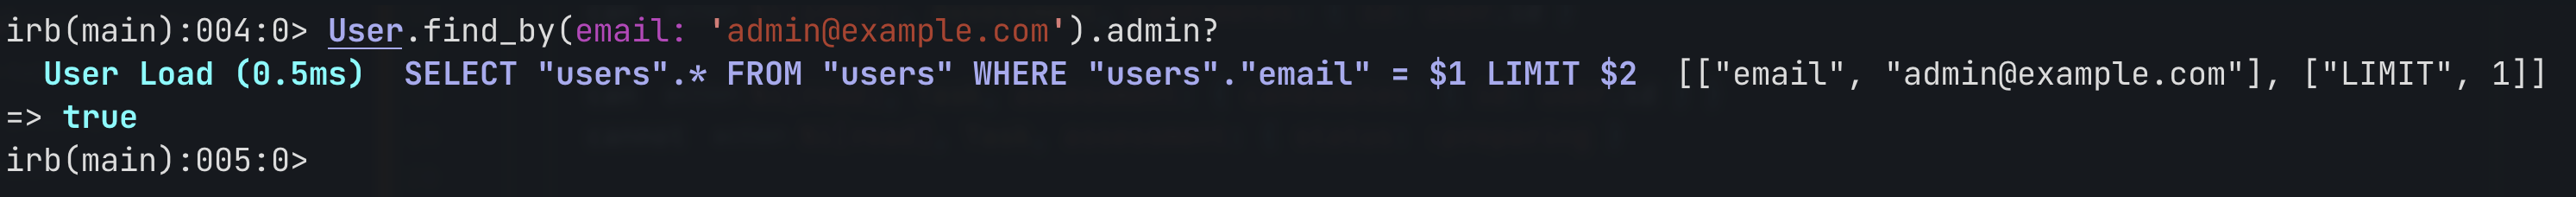
\includegraphics[width=\textwidth]{images/enum.png}
\end{figure}

\subsection{CanCanCan}

Als Autorisierungssystem wird, wie in \ref{sec:authorization} entschieden wurde, das \enquote{CanCanCan} Gem eingesetzt.
Dieses generiert nach der Installation eine Konfigurationsdatei \emph{app/models/abilities.rb}, in der
den Benutzern, basierend auf deren Rollen, sogenannte \enquote{Abilities} zugeteilt werden können.

Eine Ability-Definition kann grundsätzlich in drei Teile aufgeteilt werden und sagt gewissermassen aus: 
\emph{was darf ich?}, \emph{auf welcher Ressource darf ich?} und \emph{unter welchen Bedingungen darf ich?}

\begin{codebox}
\begin{minted}{ruby}
def candidate_abilities(user)
  can :index, Assessment, candidates: { id: user.id }

  can :read, Task, assessment: { candidates: { id: user.id } }
  cannot :read, Task, assessment: { status: :preparing }

  can :create, Solution, task: { assessment: { status: :open } }
  can :read, Solution, user_id: user.id
  can :update, Solution, user_id: user.id, task: { assessment: { status: :open } }

  can :read, Comment, solution: { user_id: user.id }
end
\end{minted}
\end{codebox}

Ein \mintinline{ruby}{:candidate} kann dementsprechend:
\begin{itemize}
  \item Nur die Assessments sehen, zu denen dieser auch Eingeladen wurde
  \item Tasks ansehen, allerdings erst, wenn das Assessment durch einen Admin gestartet wurde
  \item Lösungen erstellen, einsehen und bearbeiten, jedoch nur die eigenen
  \item Korrektur-Kommentare zu dem abgegebenen Lösungen sehen
\end{itemize}

\newpage

Ein Benutzer mit der Rolle \mintinline{ruby}{:admin} ist zu fast allem berechtigt, jedoch kann dieser:
\begin{itemize}
  \item Keine Lösungen erstellen oder bearbeiten
  \item Das Assessment und die Aufgaben nicht editieren, wenn dieses bereits gestartet wurde
\end{itemize}

\begin{codebox}
\begin{minted}{ruby}
def admin_abilities(_user)
  can :manage, :all

  cannot :edit, Assessment, status: %i[open reviewing closed]
  cannot %i[create update destroy], Task, assessment: { status: %i[open reviewing closed] }
  cannot %i[create update], Solution
end
\end{minted}
\end{codebox}
  
Die mitgelieferten Controller-Helper \mintinline{ruby}{load_resource} und \mintinline{ruby}{authorize_resource} erleichtern 
das Autorisieren der einzelnen Ressourcen und wurden daher in allen Controller-Klassen eingesetzt. Dadurch ist auch ein Grossteil vom \gls{boilerplate} Code
in den Controllern weggefallen.

Die Helper agieren wie eine \mintinline{ruby}{before_action} und werden daher vor jeder Action in den Controllern ausgeführt.
Grundsätzlich machen sie Folgendes:

\begin{enumerate}
  \item Autorisieren und laden nur die Objekte, die der Benutzer auch sehen darf
  \item Setzten automatisch die entsprechenden Instanzvariablen
\end{enumerate}

Es können auch, dem Routing entsprechend, mehrere Ressourcen geladen werden:
\begin{codebox}
\begin{minted}{ruby}
class TasksController < ApplicationController
  load_and_authorize_resource :assessment
  load_and_authorize_resource through: :assessment
  ...
end
\end{minted}
\end{codebox}

In den Views werden dann den Berechtigungen entsprechend einzelne Bedienelemente ein- oder ausgeblendet.
So wird beispielsweise auf der Assessment-Index Seite der Create-Button für Bewerber ausgeblendet, da diese keines
erstellen können:

\begin{codebox}
\begin{minted}{ruby}
- if can?(:create, Assessment)
  = link_to new_assessment_path(@assessment), class: 'btn btn-primary' do
    i.bi-plus-lg.me-2
    = t('buttons.crud.assessment.create')
\end{minted}
\end{codebox}

Durch CanCanCan konnten viele Views wiederverwendet werden und es mussten keine Extra-Seiten für die verschiedenen Rollen
erstellt werden. So werden beispielsweise auf der Seite, auf der das Assessment gelöst wird, alle
\emph{Solutions} über die entsprechende Instanzvariable gerendert. 

So sieht zwar jeder Benutzer nur seine eigene Lösung, der Admin hingegen kann alle sehen. 
So kann dieselbe Seite für das Lösen und Korrigieren eines Assessments verwendet werden.

\begin{codebox}
\begin{minted}{ruby}
= render @solutions
\end{minted}
\end{codebox}


\section{Assessment-Einladungen}

\subsection{Hinzufügen zum Assessment}

Durch den Admin sollen Bewerber per E-Mail-Adresse zu einem Assessment eingeladen werden können. Dazu wird
das \enquote{devise\_invitable} Gem verwendet, welches perfekt mit dem verwendeten Authentifizierungssystem zusammenspielt.

Durch die Installation werden automatisch die benötigten Felder auf der \emph{user} Tabelle durch eine ActiveRecord Datenbankmigration 
erstellt. Dann kann die Bibliothek wie eine Devise-Strategy gehandhabt werden:

\begin{codebox}
\begin{minted}{ruby}
class User < ApplicationRecord
  devise :invitable, ...
end
\end{minted}
\end{codebox}

Das Gem dient lediglich als eine Grundlage und muss für den geforderten Use-Case entsprechend angepasst werden.
Denn standardmässig sind nur \enquote{globale} Einladungen möglich.

Es gibt zwei Fälle die eintreten können:
\begin{itemize}
  \item Der Benutzer existiert noch nicht und muss sich erst noch einen neuen Account erstellen
  \item Der Benutzer hat schonmal an einem Assessment teilgenommen und existiert bereits
\end{itemize}

Es wurde ein eigener \emph{invitations\_controller.rb} geschrieben, dessen \emph{create} Action zuerst überprüft, ob ein Benutzer
mit der angegebenen E-Mail-Adresse bereits in der Datenbank existiert. Wenn nicht, wird über die devise\_invitable Funtkion \mintinline{ruby}{User.invite!} 
ein neuer Benutzer erstellt und automatisch ein \emph{invitation\_token} hinterlegt. Über einen Link, der diesen Token als GET-Parmaeter beinhaltet,
kann der Benutzer sich später selbstständig ein Passwort setzen.

\begin{codebox}
\begin{minted}{ruby}
@user = User.find_by(email: params[:email]) ||
        User.invite!({ email: params[:email], skip_invitation: true }, current_user)
@user.invite_to(@assessment)
\end{minted}
\end{codebox}

\begin{codebox}
\begin{minted}{ruby}
def invite_to(assessment)
  errors.add(:email, :already_in_assessment) and return if assessment.candidates.exists?(id)
  
  assessments << assessment
  send_assessment_invitation(assessment)
end
\end{minted}
\end{codebox}

Im Anschluss wird das Assessment über den Shovel-Operator \mintinline{ruby}{<<} zu den Assessments des Benutzers
hinzugefügt und eine E-Mail wird versendet.

\newpage

\subsection{E-Mail Benachrichtigungen}

Die besagte Einladungs-E-Mail wird über eine ActionMailer Klasse versendet.

\begin{codebox}
\begin{minted}{ruby}
def assessment_invitation(recipient, assessment, invitation_token)
  @invitation_token = invitation_token
  @recipient = recipient
  @assessment = assessment

  mail(to: @recipient.email,
        subject: t('invitation_mailer.assessment_invitation.subject'),
        reply_to: User.where(role: User.roles[:admin]).pluck(:email))
end
\end{minted}
\end{codebox}

Das E-Mail Template beinhaltet neben den generellen Informationen zu dem Assessment auch einen Invite-Link, über den
sich der eingeladene Benutzer einen Account erstellen kann. Dieser wird allerdings nur gerendert, wenn noch kein Account existiert.
So kann das selbe E-Mail für beide Fälle verwendet werden.

\begin{codebox}
\begin{minted}{ruby}
- if @invitation_token.present?
  p = link_to t('devise.mailer.invitation_instructions.accept'),
      accept_user_invitation_url(invitation_token: @invitation_token)
\end{minted}
\end{codebox}


\section{File-Upload}

Als Bewerber können die Lösungen zu den einzelnen Aufgaben des Assessments in Form von Dateien abgegeben werden, wobei
es sich meistens um Programmcode oder Bilder handelt. Dazu wird ein File-Upload benötigt, der in neueren Ruby on Rails Versionen über die mitgelieferte \emph{ActiveStorage} Bibliothek relativ einfach Integriert werden kann. 
ActiveStorage ist perfekt für die Cloud vorbereitet und die Integration von Amazon S3 ist bereits vorhanden. Die Konfiguration von ActiveStorage erfolgt über eine YAML-Datei.

\begin{figure}[H]
\begin{codebox}
\begin{minted}{yaml}
test:
  service: Disk
  root: <%= Rails.root.join("tmp/storage") %>

local:
  service: Disk
  root: <%= Rails.root.join("storage") %>

amazon:
  service: S3
  access_key_id: <%= ENV['AWS_S3_ACCESS_KEY_ID'] %>
  secret_access_key: <%= ENV['AWS_S3_SECRET_ACCESS_KEY'] %>
  bucket: <%= ENV['AWS_S3_BUCKET'] %>
  region: "eu-central-1"
\end{minted}
\end{codebox}
\caption{\label{fig:active-storage-config}Konfiguration von ActiveStorage über das \emph{config/storage.yml}}
\end{figure}

Für jedes Enviroment (development/test/production) kann dann Konfiguriert werden, was für ein Storage-Service verwendet werden soll.
Dazu wird z.B für Tests das lokale Verzeichnis \emph{tmp/storage} verwendet, welches nicht in das \gls{vcs} eingecheckt wird. So kann das
Upload-Feature überall genutzt werden und es wird keine dedizierte S3 Testinstanz benötigt.

Wie bereits im Diagramm \ref{fig:erd} ersichtlich, verwendet ActiveStorage gewisse Tabellen in der Datenbank, um die Uploads zu verwalten.
Sowohl der Schlüssel, der auf die eigentliche Datei im S3 verweist als auch sämtliche Metadaten wie Name, Dateigrösse oder Inhaltstyp werden in einem \emph{active\_storage\_blobs} gespeichert.
Die \emph{active\_storage\_attachments} Tabelle agiert als eine polymorphe Join-Tabelle, welche Referenzen auf ein Blob und das eigentliche Objekt (z.B auf die \emph{solution}) enthält. 
So sind mehrere Arten von Attachment-Beziehungen für ein einziges Model möglich.

Nun soll es möglich sein, mehrere Dateien zu einer \emph{solution} hochzuladen. Durch das alleinige Hinzufügen der \emph{has\_many\_attached} Funktion in das Model,
können nun Dateien über ein dediziertes Formularfeld hochgeladen werden. Damit dies auch mit mehreren Dateien auf einmal möglich ist,
wird das \emph{multiple} HTML-Attribut auf dem Input-Feld verwendet. 

\begin{codebox}
\begin{minted}{ruby}
class Solution < ApplicationRecord
  has_many_attached :uploads
  
  ...
end
\end{minted}
\end{codebox}

\begin{codebox}
\begin{minted}{ruby}
= simple_form_for([@task, @solution]) do |f|
    = f.input :uploads, input_html: { multiple: true }
    = f.button :submit
\end{minted}
\end{codebox}

Das Formular wird dann, wie man in der Formulardefinition erkennen kann, unter einen Task \enquote{genested} und auf dessen Detail-Seite gerendert.
So würde dieses Formular beispielsweise auf \emph{/tasks/275/solutions} posten und so eine neue Lösung für die entsprechende Aufgabe erstellen.

\begin{figure}[H]
  \centering
  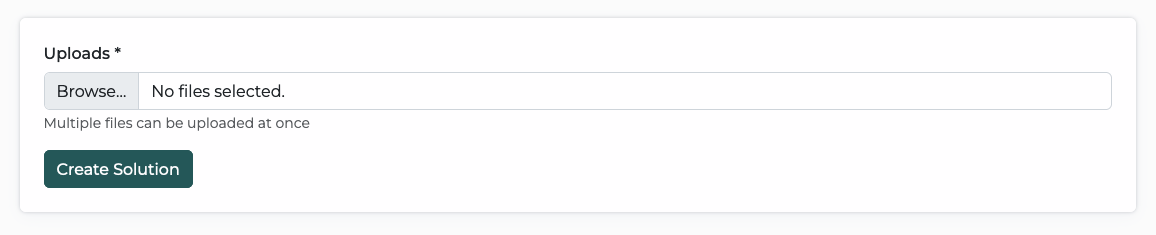
\includegraphics[width=\textwidth]{images/upload.png}
  \caption{\label{fig:solution-create}Formular für das Hochladen einer Lösung}
\end{figure}


\section{Formatierte Textinhalte}

Die Aufgaben und Korrektur-Kommentare sollen durch formatierten Text strukturiert dargestellt werden.
Dazu wird die bereits angesprochene \enquote{ActionText} Bibliothek verwendet, die ebenfalls standardmässig mit Ruby on Rails mitgeliefert wird.
Diese enthält neben einigen praktischen Helpern auch den JS Trix-Editor, der alles von der Formatierung über Links, Zitate und Listen bis hin zu eingebetteten Bildern übernimmt. 

Der vom Trix-Editor generierte Rich-Text-Inhalt wird im HTML-Format gespeichert und eingebettete Bilder (oder andere Anhänge) werden automatisch durch ActiveStorage verwaltet.

Über den generator-command \mintinline{bash}{rails g action_text:install} werden die notwendigen migrationen erstellt und
der Trix-Editor wird über den yarn JS Package-Manager installiert. Dann wurde lediglich die \mintinline{ruby}{has_rich_text} Funktion
zu dem Model hinzugefügt. 

\begin{codebox}
\begin{minted}{ruby}
class Task < ApplicationRecord
  has_rich_text :body
  
  ...
end
\end{minted}
\end{codebox}

\begin{codebox}
\begin{minted}{ruby}
= simple_form_for [@assessment, @task] do |f|
    = f.input :body, as: :rich_text_area
    = f.button :submit
\end{minted}
\end{codebox}

Rich-Text Inhalte wurden sowohl für die Aufgabenbeschreibung als auch die Korrektur-Kommentare umgesetzt und sehen
in den Formularen so aus:

\begin{figure}[H]
  \centering
  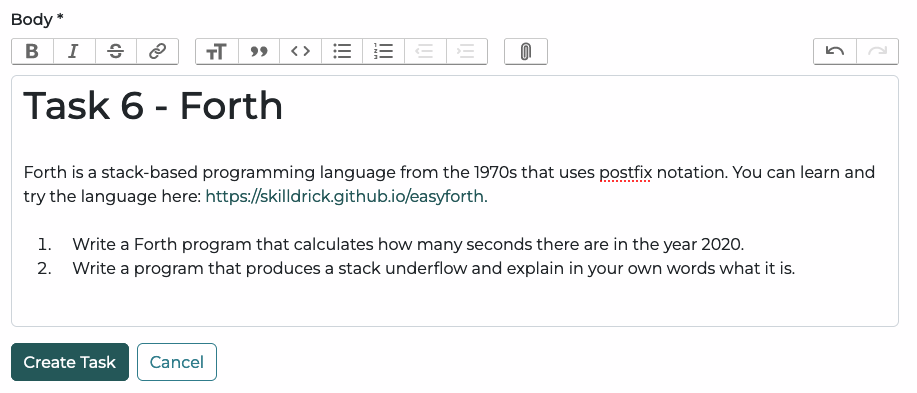
\includegraphics[width=14cm]{images/trix.png}
  \caption{Der ActionText \emph{trix} Rich-Text-Editor}
\end{figure}


\section{Zeitbegrenzung}

Nachdem das Assessment durch den Admin gestartet wurde und es seinen Zustand zu \enquote{open} gewechselt hat, wird
ein Background-Job erstellt, der das Assessment rechtzeitig beenden soll. Dieser wird auf der Produktions-Umgebung 
über das Sidekiq ActiveJob-Backend in die Warteschlange einer Redis in-memory Datenbank gestellt. 

Der Job ist sehr simpel und ruft eine einzige Funktion auf der Assessment-Instanz auf, 
die über die State-Machine dessen Zustand wechselt. 

\begin{codebox}
\begin{minted}{ruby}
class EndAssessmentJob < ApplicationJob
  queue_as :default

  def perform(assessment)
      assessment.finish!
  end
end
\end{minted}
\end{codebox}

Ausserdem soll für den Bewerber jederzeit ersichtlich sein, wie lange dieser für das Assessment Zeit hat. 
Dafür wird ein JS basierter Countdown über das Stimulus Framework implementiert, der die verbleibende Zeit runterzählt.

Der Stimulus-Controller wird hier über das \emph{data-controller} HTML-Attribut an das \mintinline{html}{<h3>} Element gebunden.
Ausserdem wird das exakte DateTime, an dem das Assessment beendet wird, im Unix-Timestamp-Format an die Controller-Klasse weitergegeben.

\begin{figure}[H]
\begin{codebox}
\begin{minted}{html}
h3(data-controller='assessment-time' data-assessment-time-end-value=@assessment.ends_at.to_i)
\end{minted}
\end{codebox}
\end{figure}

Der Timestamp kann dann im Controller als Stimulus-Value 

\begin{figure}[H]
\begin{codebox}
\begin{minted}{javascript}
export default class extends Controller {
  static values = { end: Number }

  connect () {
    this.countdownInterval = setInterval(() => {
      this.element.innerText = this.parsedTime;
    }, 1000);
  }

  disconnect () {
    clearInterval(this.countdownInterval);
  }

  get parsedTime () {
    const remainingSeconds = this.endValue * 1000 - Date.now();
    
    ...
    
    return `${hours}:${minutes}:${seconds}`;
  }

  ...
}
\end{minted}
\end{codebox}
\end{figure}

\begin{figure}[H]
  \centering
  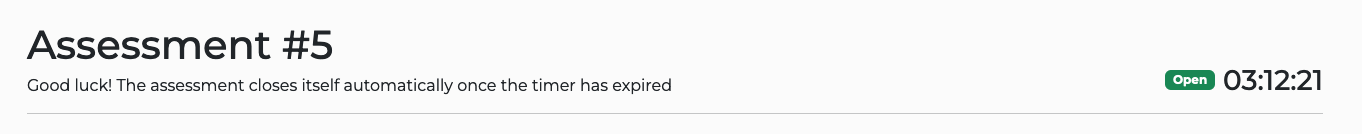
\includegraphics[width=\textwidth]{images/countdown.png}
\end{figure}


\section{User-Interface}

Für die Umsetzung des UI wurde das \enquote{Bootstrap} CSS-Framework verwendet. Ausserdem wurden alle
HTML-Templates in der Ruby SLIM templating-language geschrieben, 
welche eine stark vereinfachte Syntax ohne \enquote{Brackets} und ohne \enquote{Closing-Tags} bietet.

Durch diese zwei Mittel und mit der Hilfe der in der Planungsphase erstellten Mockups \ref{sec:mockups}, konnte das UI
rasch umgesetzt werden und ist durch eine klare farbliche Hierarchie ergonomisch strukturiert. Wo nötig, wurden auch
Icons eingesetzt.

\subsection{Assessments erstellen und verwalten}

\begin{figure}[H]
  \centering
  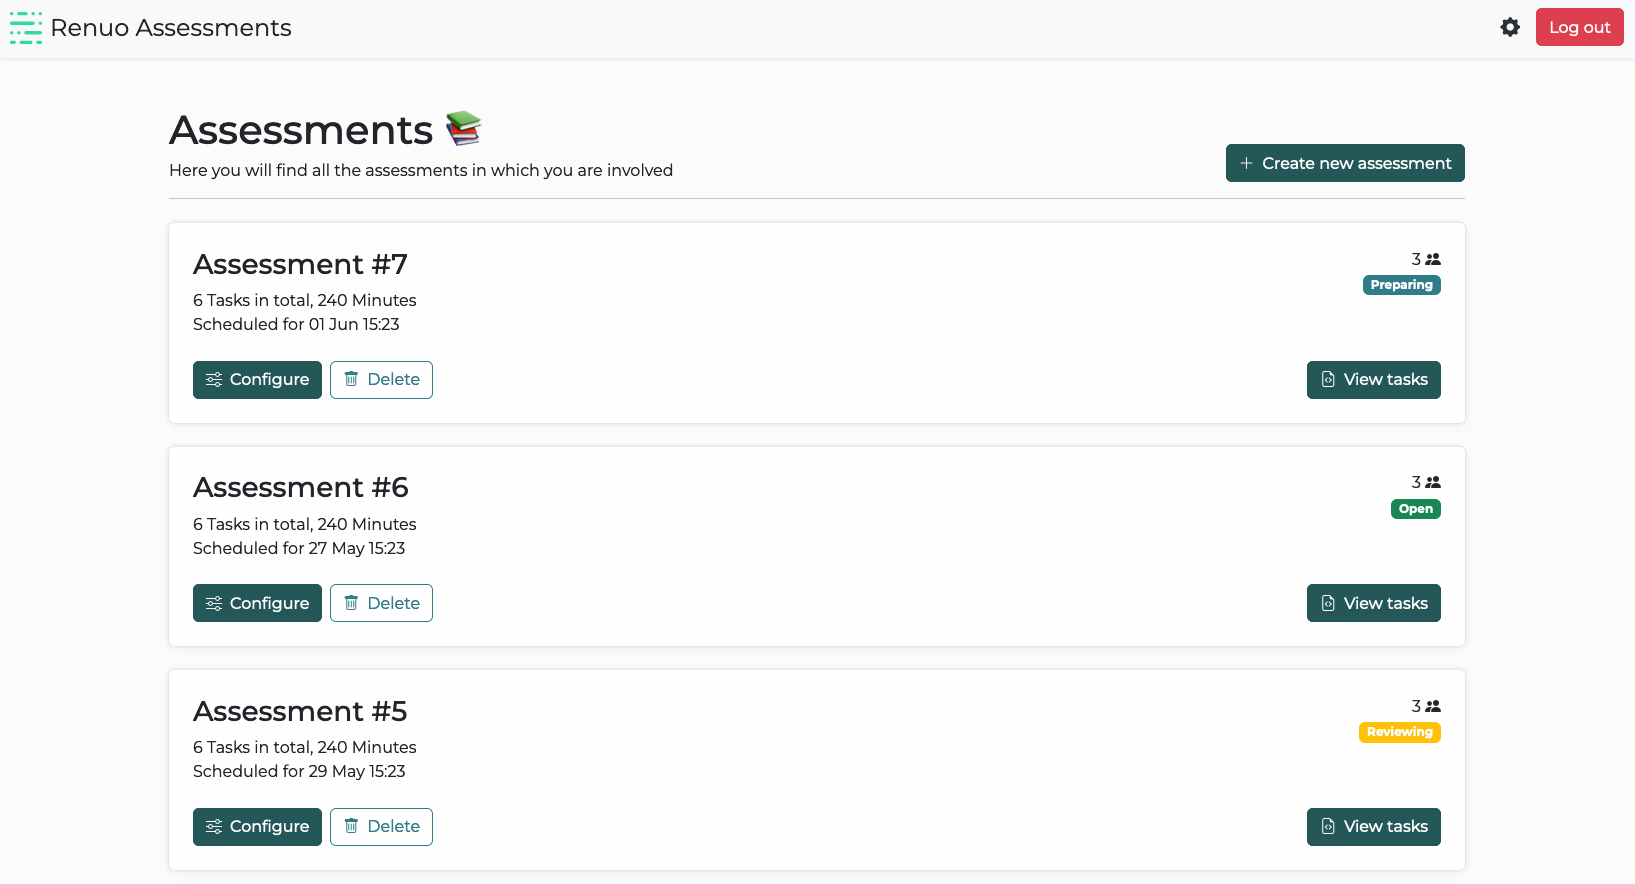
\includegraphics[width=\textwidth]{images/ui/assessments-index.png}
  \caption{\label{fig:assessments-index}Index-Seite, die alle Assessments auflistet}
\end{figure}

\begin{figure}[H]
  \centering
  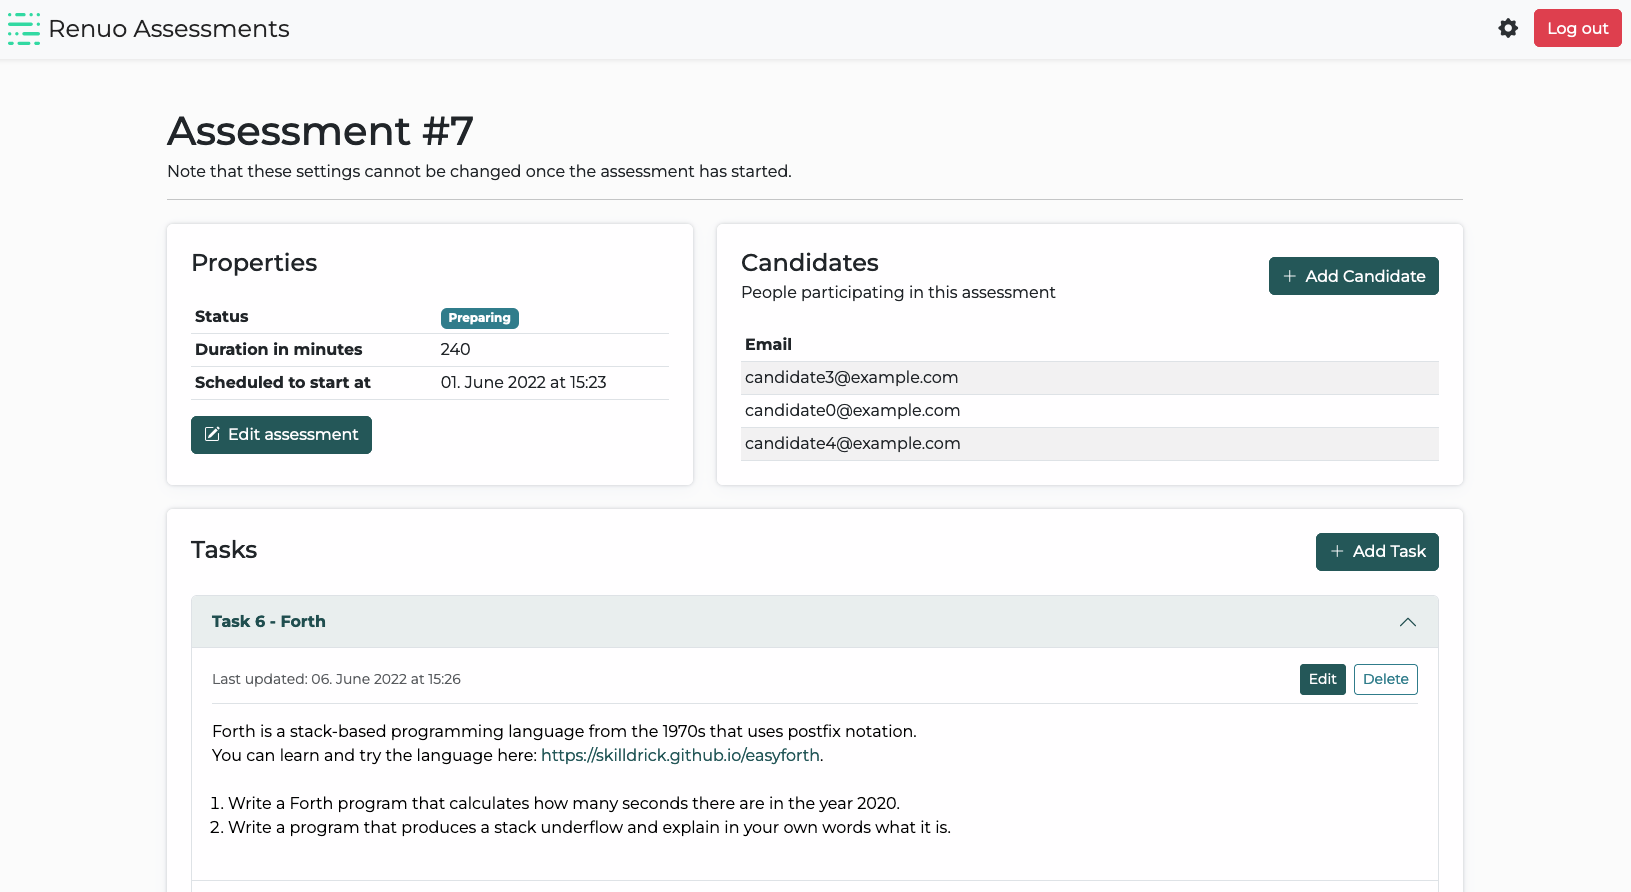
\includegraphics[width=\textwidth]{images/ui/assessments-edit.png}
  \caption{\label{fig:assessments-edit}Konfiguration des Assessments}
\end{figure}

\subsection{Assessments lösen}

\begin{figure}[H]
  \centering
  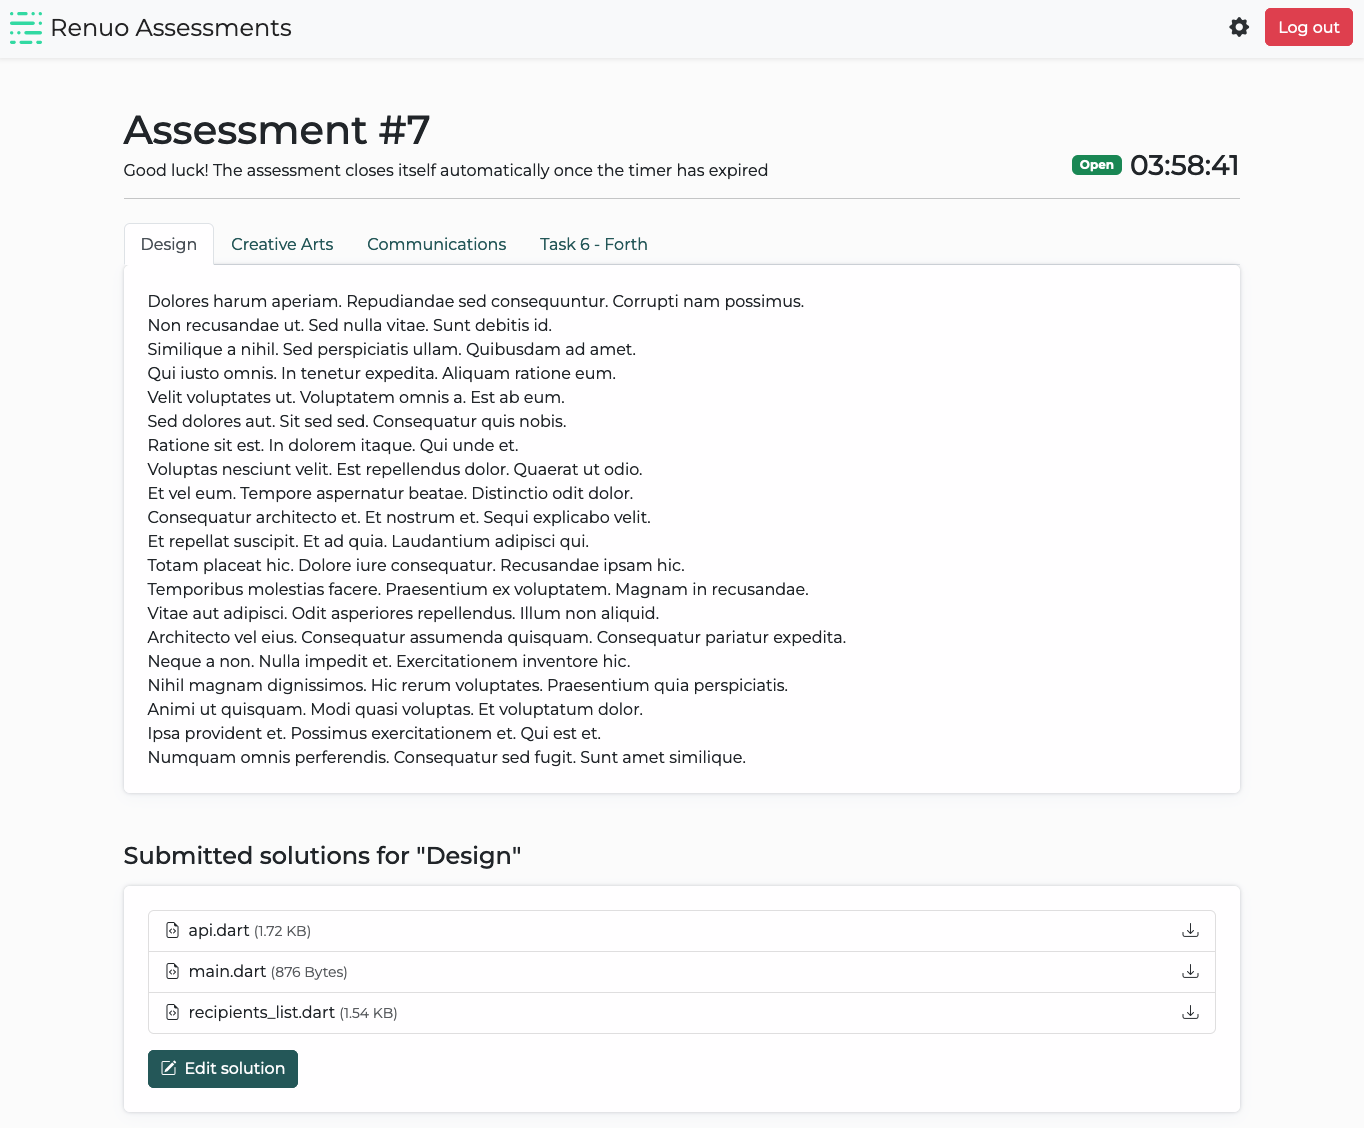
\includegraphics[width=14cm]{images/ui/solve-assessment.png}
  \caption{\label{fig:solve-assessment}Lösen eines Assessments}
\end{figure}


\subsection{Assessments korrigieren}

\begin{figure}[H]
  \centering
  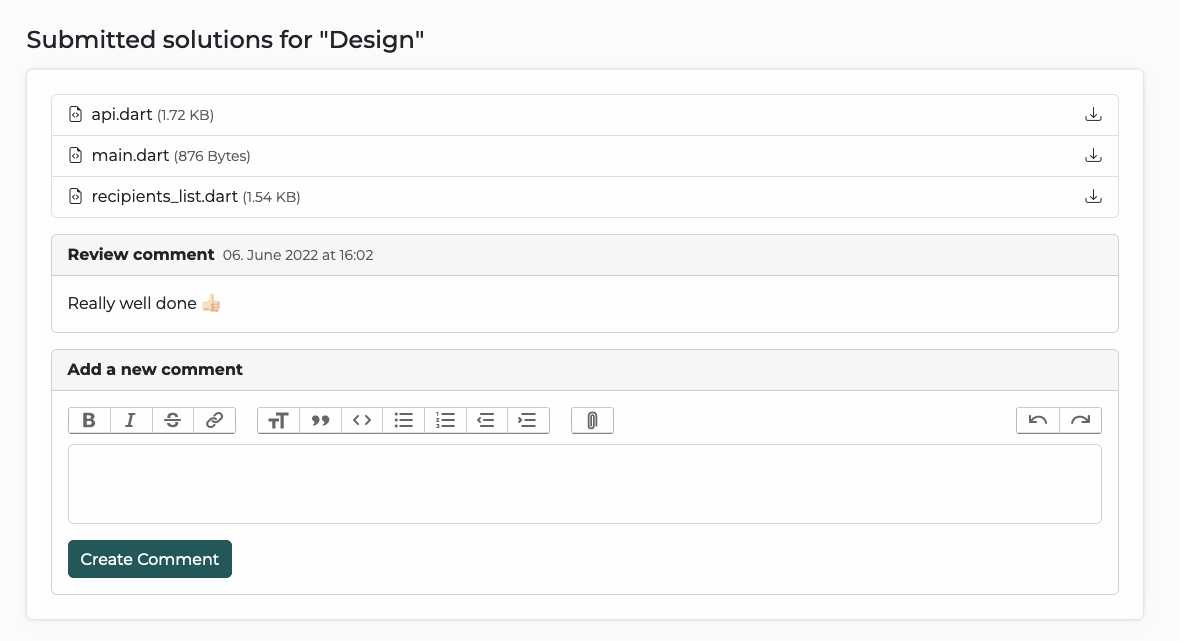
\includegraphics[width=14cm]{images/ui/review-comments.png}
  \caption{\label{fig:review-comments}Assessment auswerten}
\end{figure}


\section{Validierungen}

\section{Code-Style}
